\documentclass{article}
\usepackage{graphicx}
\graphicspath{{res/}}
\usepackage{subcaption}
\usepackage{url}
\usepackage{afterpage}


\title{ Latex Figures}
\date{2020/11/09}
\author{Steven Huang}

\begin{document}
\pagenumbering{gobble}
\maketitle
\newpage
\pagenumbering{arabic}

\section{figure1}
Hello World!
\section{figure2}
\begin{figure}[htb!] %[h!]
  \centering
  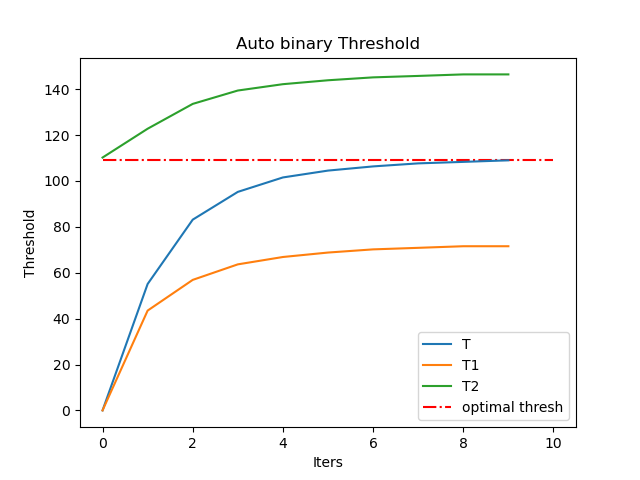
\includegraphics[width=0.5\linewidth]{autoThres.png}
  \caption{Auto binary threshold method.}
  \label{fig:bin1}
\end{figure}

\begin{figure}[htb!] %[h!]
  \centering
  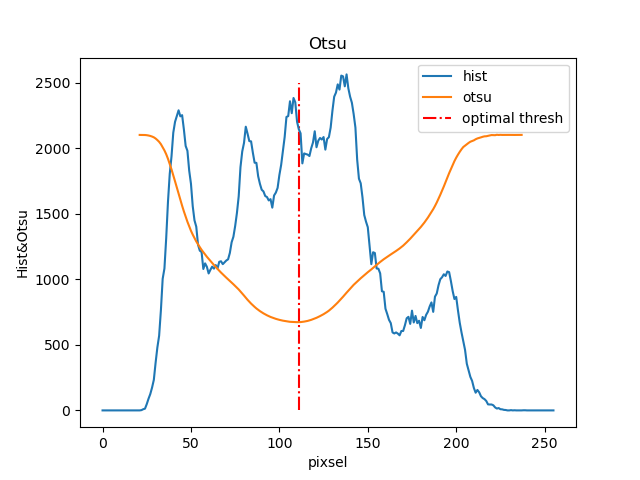
\includegraphics[width=0.5\linewidth]{otsu.png}
  \caption{Otsu threshold method.}
  \label{fig:Otsu1}
\end{figure}

Figure \ref{fig:bin1} shows a boat. 
Figure \ref{fig:Otsu1} shows the otsu method.

\section{sub-figure1}
Here will show tow images next to each other.

\begin{figure}[htb!] %[h!]
  \centering
  \begin{subfigure}[b]{0.45\linewidth}
    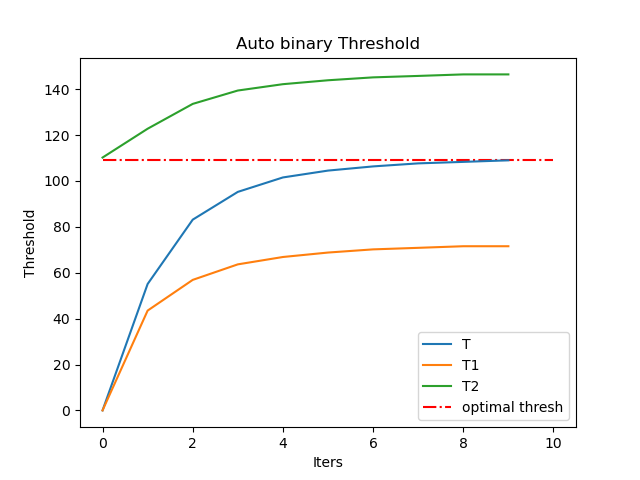
\includegraphics[width=\linewidth]{autoThres.png}
    \caption{Auto threshold.}
  \end{subfigure}
  \begin{subfigure}[b]{0.45\linewidth}
    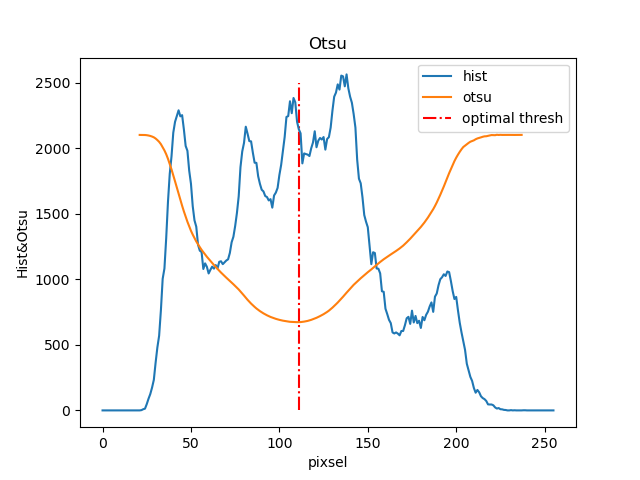
\includegraphics[width=\linewidth]{otsu.png}
    \caption{Otsu method.}
  \end{subfigure}
  \caption{The method for image binary segmentation.}
  \label{fig:imageSeg}
\end{figure}

\section{sub-figure2}
More conloex align figures.More conloex align figures.More conloex align figures.More conloex align figures.More conloex align figures.More conloex align figures.More conloex align figures.More conloex align figures.More conloex align figures.More conloex align figures.More conloex align figures.More conloex align figures.More conloex align figures.More conloex align figures.
\begin{figure}[htb!] %[h!]
  \centering
  \begin{subfigure}[b]{0.4\linewidth}
    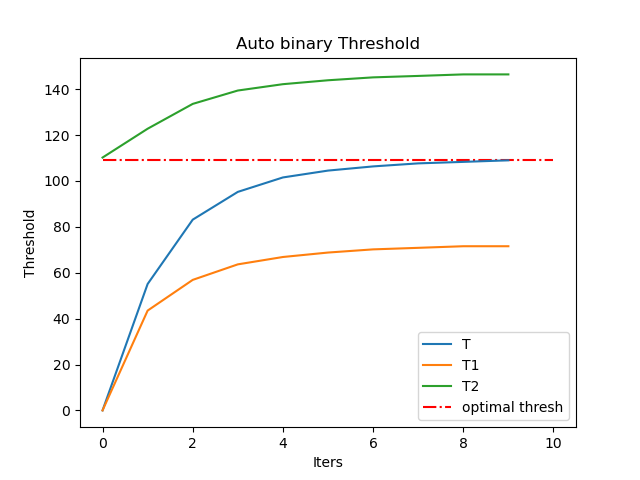
\includegraphics[width=\linewidth]{autoThres.png}
     \caption{Coffee.}
  \end{subfigure}
  \begin{subfigure}[b]{0.4\linewidth}
    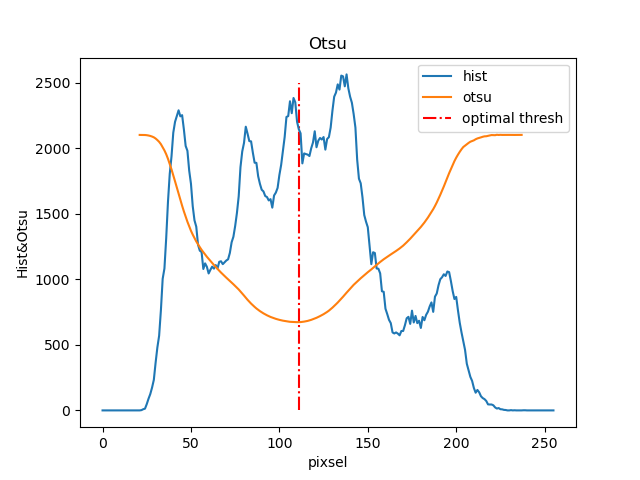
\includegraphics[width=\linewidth]{otsu.png}
    \caption{More coffee.}
  \end{subfigure}
  \begin{subfigure}[b]{0.4\linewidth}
    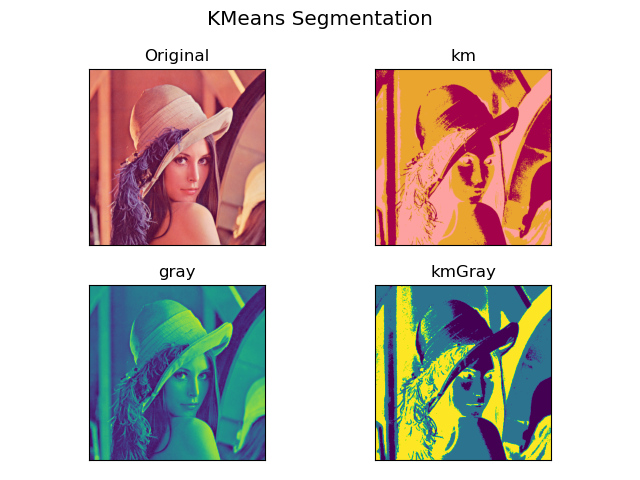
\includegraphics[width=\linewidth]{kMeans.png}
    \caption{Too much coffee.}
  \end{subfigure}
  \begin{subfigure}[b]{0.4\linewidth}
    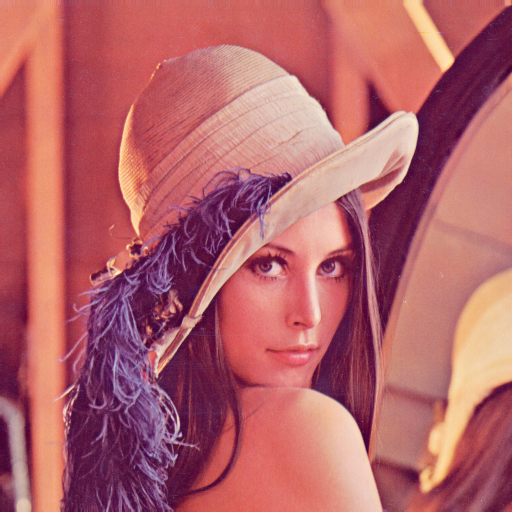
\includegraphics[width=\linewidth]{Lenna.png}
    \caption{Too much coffee.}
  \end{subfigure}
  \caption{The same cup of coffee. Multiple times.}
  \label{fig:coffee3}
\end{figure}

\newpage

\section{caption footnode}
And this is the Yolo url\footnote{\label{bbb}\url{https://www.google.com/}}.

\begin{figure}[htb!]
  \begin{center}
    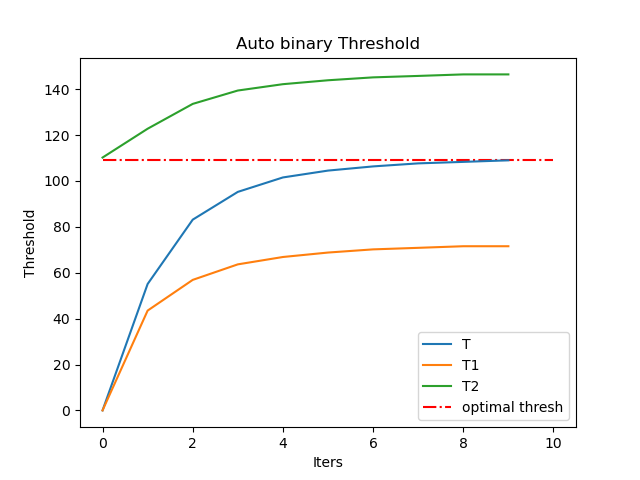
\includegraphics[scale=0.6]{autoThres.png}
      \caption[The LOF caption]{Lorem ipsum. {This image is taken from somewhere\footnote{Source: \url{http://www.example.com/the_image.png}}}}
    \label{fig:cited_img}
    \end{center}
\end{figure}

\begin{figure}
   \centering
    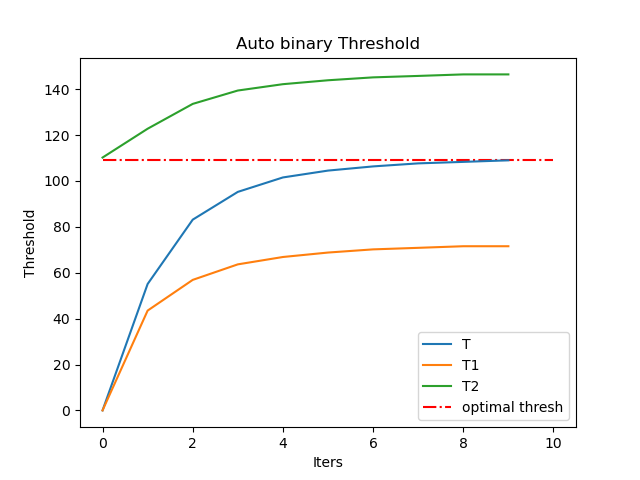
\includegraphics[scale=0.6]{autoThres.png}
   \caption[Caption for LOF]{Real caption\protect\footnotemark}
\end{figure}
%\footnotetext{autoThres}

\begin{figure}
   \centering
    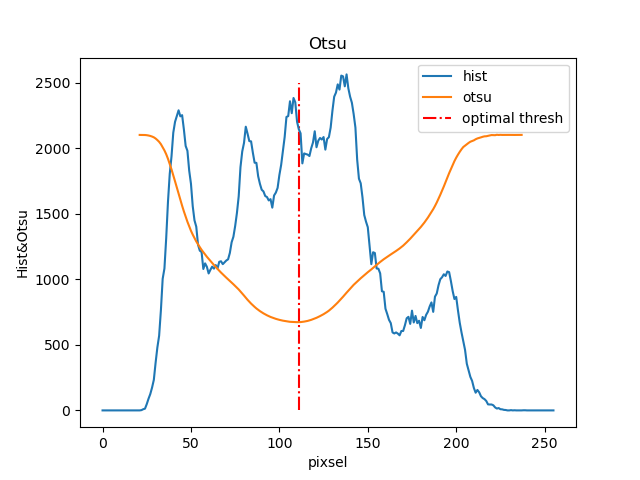
\includegraphics[scale=0.6]{otsu.png}
   \caption[Caption for LOF]{Real caption\protect\footnotemark}
\end{figure}
\footnotetext{otsu}

\end{document}